%*----------- SLIDE -------------------------------------------------------------
\begin{frame}[t]{Hardware}

	\begin{itemize}
        \item Circuito utilizado como os controles do jogo
	\item Os potenciômetros controlam as barras (paddles)
	\item Os botões fazem a transição de telas e pausam o jogo.
    \end{itemize}
   
	\vspace{0.3cm}
	\begin{columns}
		% Column 1
		\begin{column}{0.5\textwidth}
			\begin{figure}
				\centering
					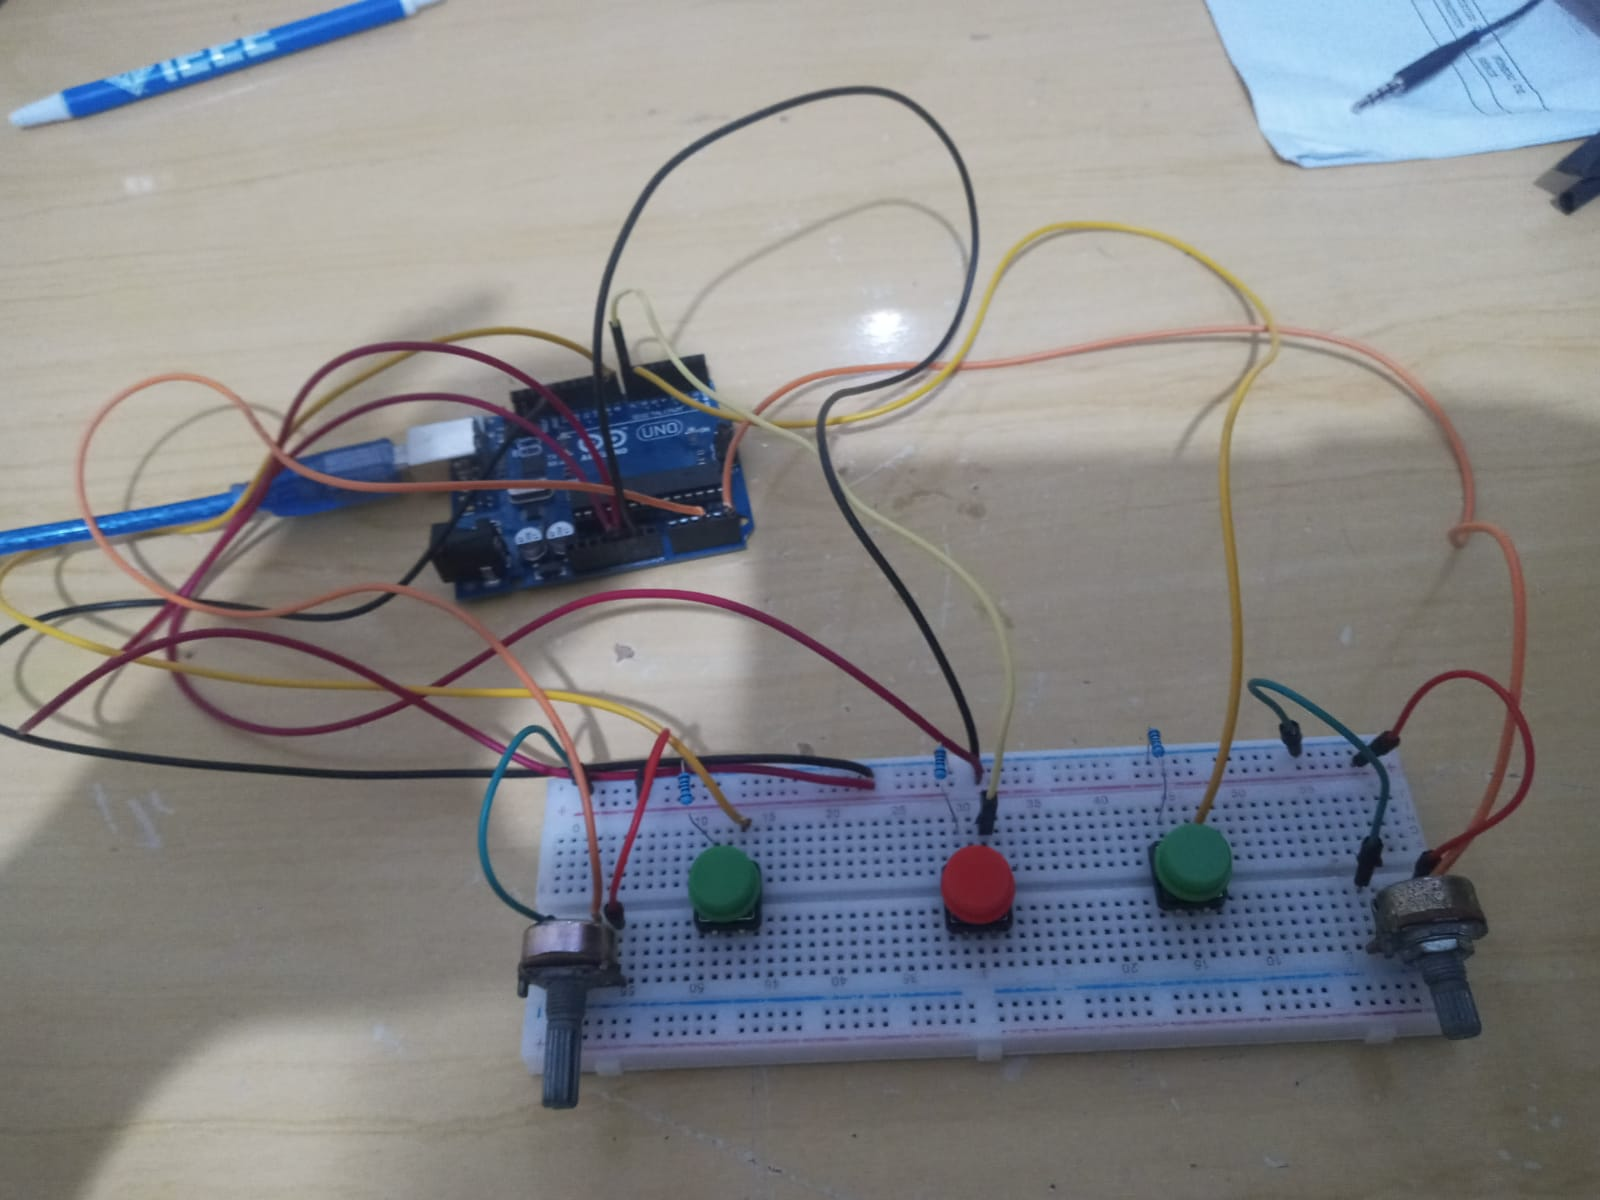
\includegraphics[width=0.6\textwidth]{circuito}
			\end{figure}
		\end{column}
			% Column 2    
			\begin{column}{0.7\textwidth}
				\begin{figure}
					\centering
						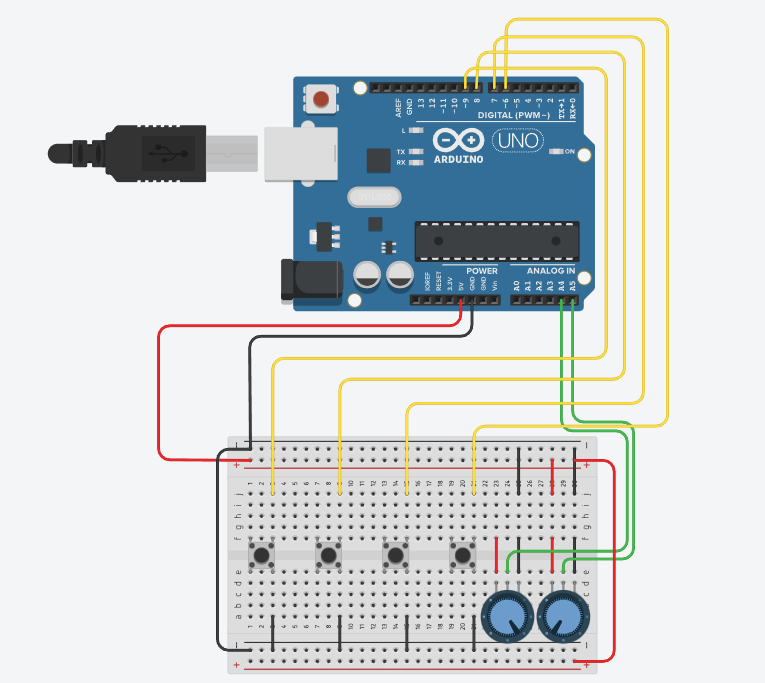
\includegraphics[width=0.4\textwidth]{esquematico-arduino}
				\end{figure}
			\end{column}
		\end{columns}

%*----------- notes
    \note[item]{Notes can help you to remember important information. Turn on the notes option.}
\end{frame}
%-
%*----------- SLIDE -------------------------------------------------------------
\begin{frame}[c]{Hardware - Controles}
 
  \begin{itemize}
      \item Modelos Impressos 3D para acomodar os botões e potenciômetros do circuito.
	\item Estes também são mais cômodos para os jogadores
    \end{itemize}
\vspace{0.3cm}
\begin{columns}
	% Column 1
	\begin{column}{0.4\textwidth}
		\begin{figure}
			\centering
    			\includegraphics[width=0.6\textwidth]{botão}
    			\caption{Os modelos impressos.}
    			%%\label{fig:question}
		\end{figure}
	\end{column}
		% Column 2    
		\begin{column}{0.4\textwidth}
			\begin{figure}
				\centering
    				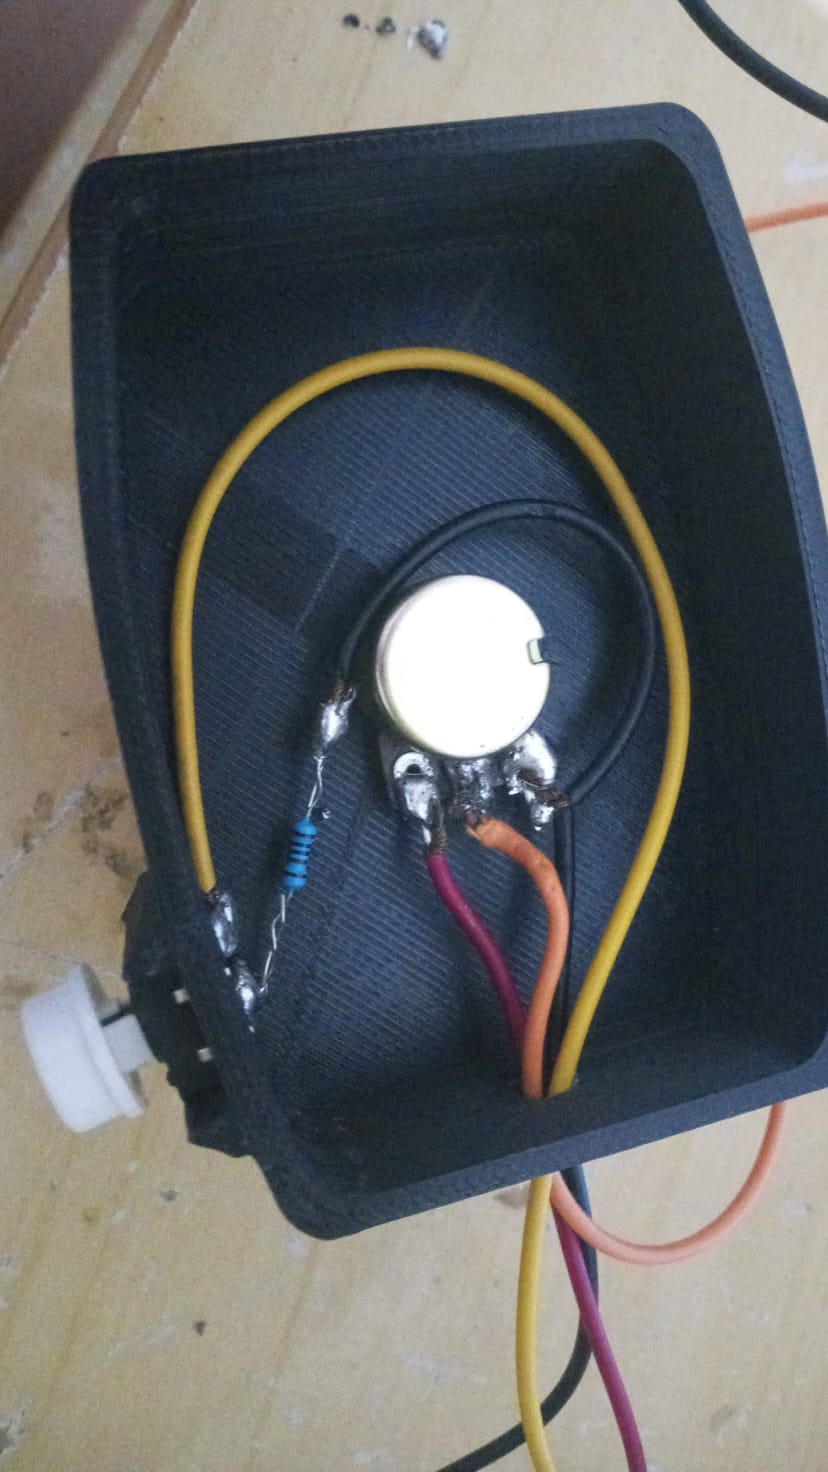
\includegraphics[width=0.4\textwidth]{solda}
    				\caption{A solda cos componentes no controle.}
    				%%\label{fig:question}
			\end{figure}
		\end{column}
	\end{columns}
%*----------- notes
    \note[item]{Notes can help you to remember important information. Turn on the notes option.}
 \end{frame}
%-
%*----------- SLIDE -------------------------------------------------------------
\begin{frame}[fragile]{Hardware - Arduino}
	 
\scriptsize
\begin{columns}
% Column 1
\begin{column}{0.5\textwidth}
	\begin{lstlisting}[language=C]
const int pot1 = A0, pot2 = A1; 
const int b01 = 8, b02 = 7; 
int v_pot1 = 0, v_pot2 = 0; 
bool v_b01,v_b02; 
int arr[10];

void setup() {
	Serial.begin(9600);
	pinMode(pot1, INPUT);
	pinMode(pot2, INPUT);
	for(int i = 7; i <= 8; i++){
	pinMode(i, INPUT_PULLUP);
	}
}
	\end{lstlisting}
\end{column}
% Column 2    
\begin{column}{0.55\textwidth}
	\begin{lstlisting}[language=C]
void loop() {

v_pot1 = map(analogRead(pot1),0,1023,0,255);
Serial.print(String(v_pot1) + "-");

v_pot2 = map(analogRead(pot2),0,1023,0,255);
Serial.print(String(v_pot2) + "-");

v_b01 = !digitalRead(b01);
v_b02 = !digitalRead(b02);

Serial.print(String(v_b01) + "-");
Serial.print(String(v_b02) + "\n");
delay(50);

}		
	\end{lstlisting}
\end{column}
\end{columns} 


%*----------- notes
    \note[item]{Notes can help you to remember important information. Turn on the notes option.}
 \end{frame}
%-
%*----------- SLIDE -------------------------------------------------------------
\begin{frame}[c]{Hardware - Arduino}
\vspace{0.2cm}
\begin{itemize}
        \item Como pode ser visto, uma string de modelo [x-x-x-x] é enviada ao Processing serialmente.
	  \item No Processing, essa string será separada em caracteres e cada um sera atribuido a sua respectiva classe.
    \end{itemize}

\begin{figure}
	\centering
    	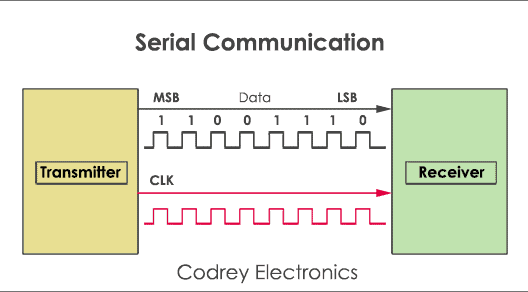
\includegraphics[width=0.4\textwidth]{serial}
    	%\caption{Representação d}
    	%%\label{fig:question}
\end{figure}

%*----------- notes
    \note[item]{Notes can help you to remember important information. Turn on the notes option.}
 \end{frame}
 %-
%*----------- SLIDE -------------------------------------------------------------
\begin{frame}[c]{Software}
	\emph {Afinal, do que consiste o jogo "P-OO-ng"?}
	\vspace{0.2cm}

\begin{itemize}
	\item Desenvolvimento do game em Processing;
	\item Menu principal, instruções e tela pause;
	\item Física da bola;
	\item Colisão com as barras;
	\item Interpretação do que o Arduino envia;
	\item Todo o desenvolvimento estético (formas, cores, etc).
\end{itemize}
    
%*----------- notes
    \note[item]{Notes can help you to remember important information. Turn on the notes option.}
 \end{frame}
 %-
%*----------- SLIDE -------------------------------------------------------------
\begin{frame}[c]{Software - Telas}
    %\transdissolve[duration=0.5]
    %\hspace*{-1cm}
\begin{itemize}
	\item Definidas através de um "switch-case".
	\item Representam a interface em que o jogador está.
	\item Com a seleção de opções, a transição é efetuada.
\end{itemize}
  
\begin{figure}
	\centering
    	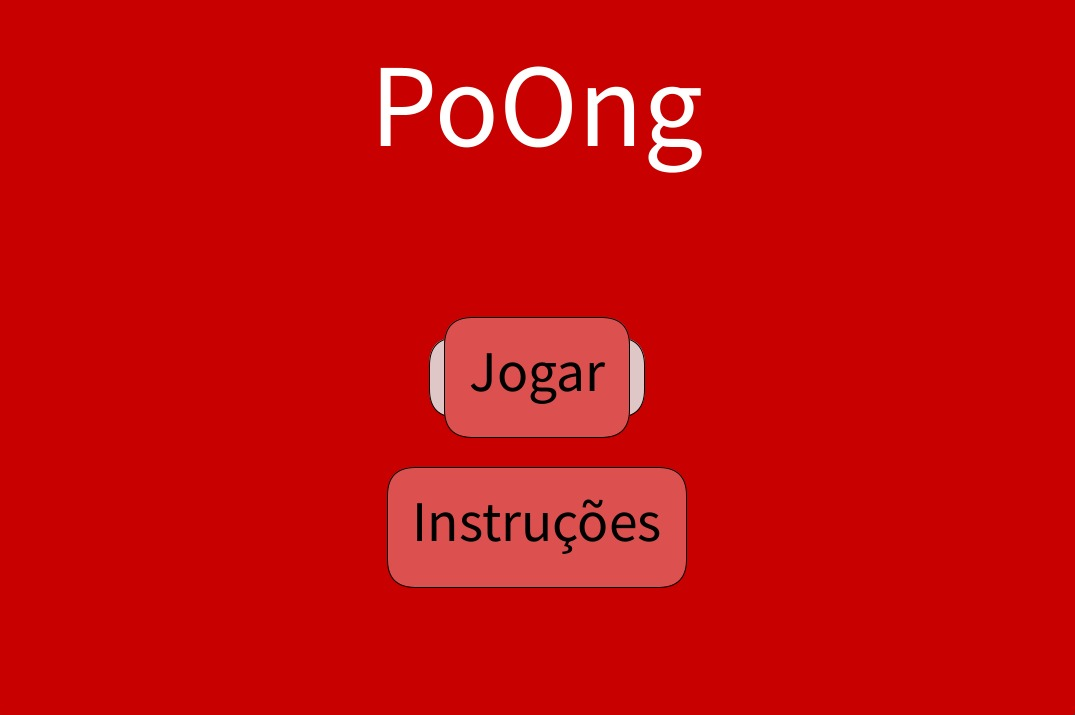
\includegraphics[width=0.4\textwidth]{tela-inicial}
    	\caption{Tela de início do jogo.}
    	%%\label{fig:question}
\end{figure}

 %*----------- notes__
    \note[item]{Notes can help you to remember important information. Turn on the notes option.}
\end{frame}
%-
%*----------- SLIDE -------------------------------------------------------------
\begin{frame}[c]{Software - Evolução da tela de início}
    
  \begin{figure}
	\centering
    	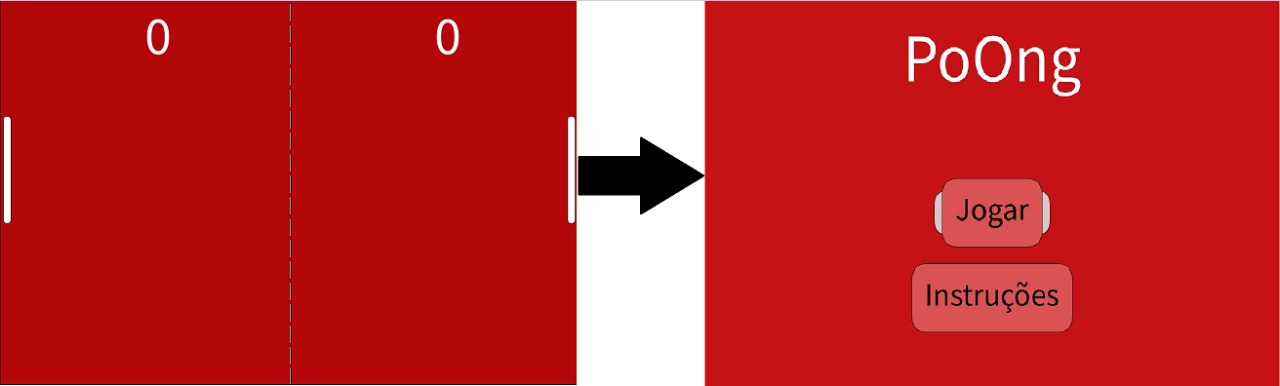
\includegraphics[width=0.7\textwidth]{melhoria}
    	\caption{Antes, quando era apenas o jogo X A tela de início criada.}
    	%%\label{fig:question}
\end{figure}


 %*----------- notes__
    \note[item]{Notes can help you to remember important information. Turn on the notes option.}
\end{frame}
%-
%*----------- SLIDE -------------------------------------------------------------
\begin{frame}[c]{Software - Tela de Instruções}
    %\transdissolve[duration=0.5]
	
	\begin{itemize}
		\item Ensina brevemente como se jogar o jogo!
	\end{itemize}
		
	  \begin{figure}
		\centering
	    	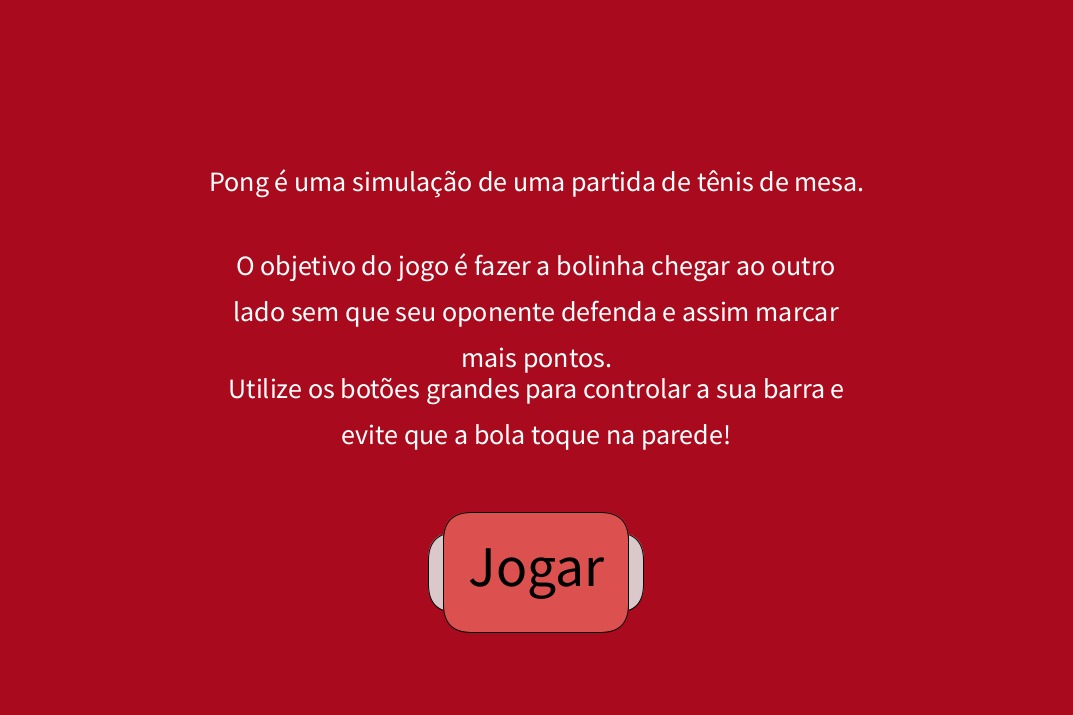
\includegraphics[width=0.5\textwidth]{instrucoes}
	    	\caption{Tela de instruções do jogo.}
	    	%%\label{fig:question}
	\end{figure}

 %*----------- notes__
    \note[item]{Notes can help you to remember important information. Turn on the notes option.}
\end{frame}
%-
%*----------- SLIDE -------------------------------------------------------------
\begin{frame}[c]{Software - Tela Pause}
    %\transdissolve[duration=0.5]
	
	\begin{itemize}
		\item Quando o botão do controle é apertado enquanto o jogo estiver sendo jogado, a tela de pause aparece, zerando a velocidade da bolinha, deixando-a imóvel até que uma das opções seja selecionada novamente.
	\end{itemize}
		
	  \begin{figure}
		\centering
	    	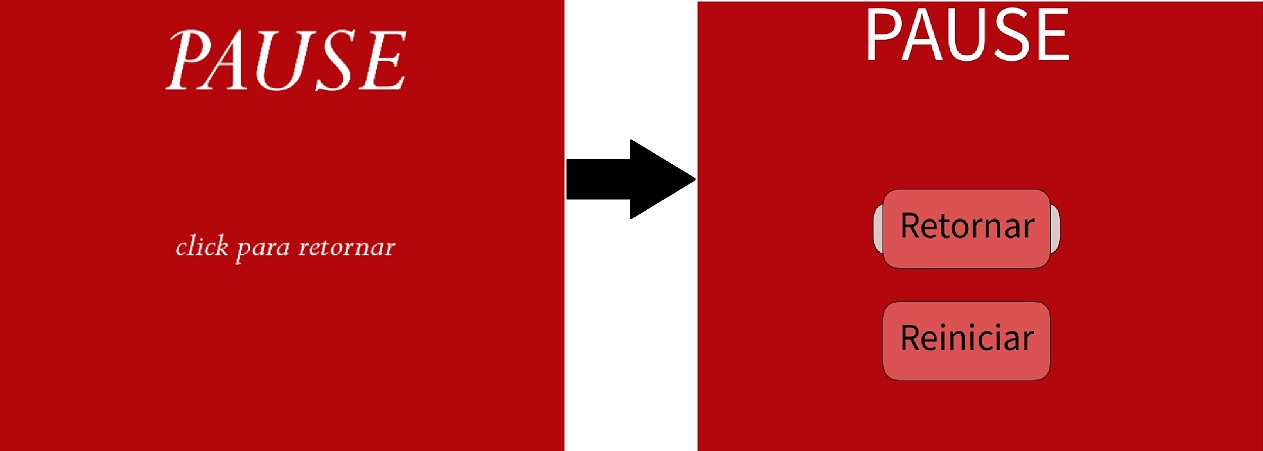
\includegraphics[width=0.6\textwidth]{pause}
	    	\caption{Tela de pause do jogo (antiga X nova).}
	    	%%\label{fig:question}
	\end{figure}

 %*----------- notes__
    \note[item]{Notes can help you to remember important information. Turn on the notes option.}
\end{frame}
%-
%*----------- SLIDE -------------------------------------------------------------
\begin{frame}[fragile]{Software - Lógica das telas}
    %\transdissolve[duration=0.5]
\emph{Exemplo da lógica para a tela inicial:}
\vspace{0.1cm}
\centering
\begin{columns}
% Column 1
\begin{column}{0.4\textwidth}
\scriptsize
\begin{lstlisting}[language=java]
switch (ordem) { // Ordena as cenas do jogo
case 0:
tela_inicial();

if (click == 0 && (botao1.indexOf('1') != -1 || botao2.indexOf('1') != -1)) click = 1;
		
if (click == 1 && (botao1.indexOf('1') == -1) && (botao2.indexOf('1') == -1)) {
		
	if (int(strBarra1) > 127 || int(strBarra2) > 127) {
		click = 4;
		ordem = 2;
	} else {
		click += 1;
		ordem = 1;
		}
	}
break;
\end{lstlisting}
\end{column}
\begin{column}{0.7\textwidth}
			.	
			\end{column}
\end{columns}
 %*----------- notes__
    \note[item]{Notes can help you to remember important information. Turn on the notes option.}
\end{frame}
%
%*----------- SLIDE -------------------------------------------------------------
\begin{frame}[c]{Software - Componentes do jogo}
    %\transdissolve[duration=0.5]
	
	\begin{figure}
		\centering
	    	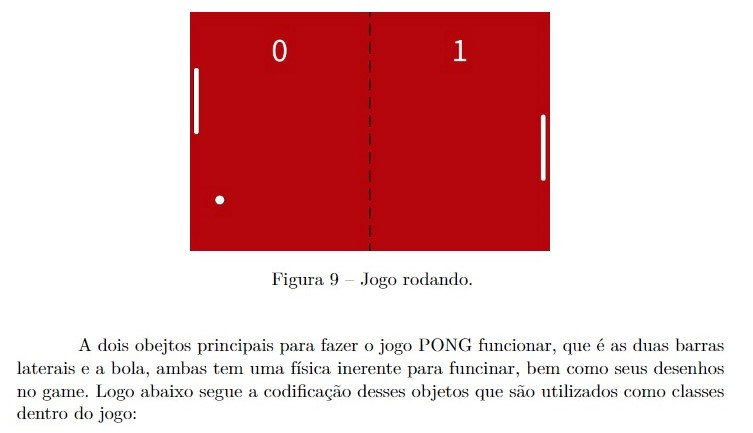
\includegraphics[width=0.8\textwidth]{componentes}
	    	%\caption{}
	    	%%\label{fig:question}
	\end{figure}


 %*----------- notes__
    \note[item]{Notes can help you to remember important information. Turn on the notes option.}
\end{frame}
%-
%-
%*----------- SLIDE -------------------------------------------------------------
\begin{frame}[c]{Software - Componentes do jogo}
    %\transdissolve[duration=0.5]
	\emph{Vamos ver com mais detalhes no artigo!}
	\href{https://github.com/Mila2k2/Desafio-03-Pong/blob/main/artigo-pong/modelo-artigo.pdf}{\beamergotobutton{Link}}


 %*----------- notes__
    \note[item]{Notes can help you to remember important information. Turn on the notes option.}
\end{frame}
%-
%*----------- SLIDE -------------------------------------------------------------
\begin{frame}[c]{Demosntração 1}
    %\transdissolve[duration=0.5]
\centering
\includemedia[
      width=0.7\linewidth,
      totalheight=0.39375\linewidth,
      activate=pageopen,
      passcontext, 
      addresource=./Source/movies/demo.mp4,
      flashvars={
      source=./Source/movies/demo.mp4
      &autoPlay=true
      &Loop=false}
      ]{\fbox{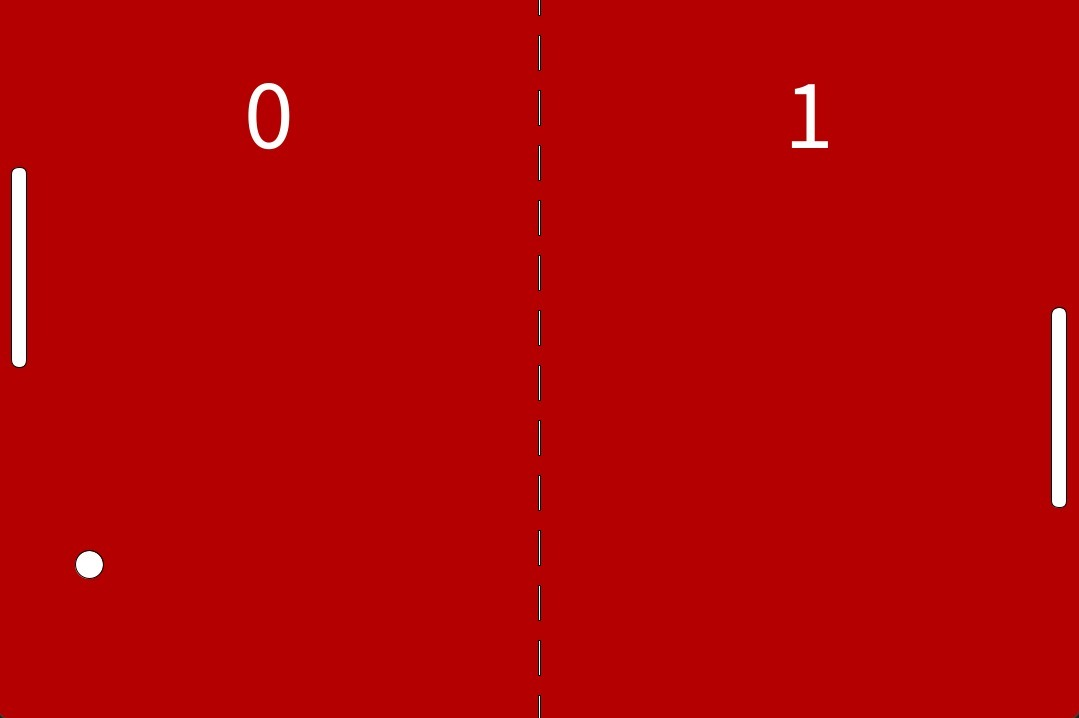
\includegraphics{rodando}}}{VPlayer.swf}

 %*----------- notes__
    \note[item]{Notes can help you to remember important information. Turn on the notes option.}
\end{frame}
%-
%-
%*----------- SLIDE -------------------------------------------------------------
\begin{frame}[c]{Demosntração 2}
    %\transdissolve[duration=0.5]
\centering
\includemedia[
      width=0.7\linewidth,
      totalheight=0.39375\linewidth,
      activate=pageopen,
      passcontext, 
      addresource=./Source/movies/demo2.mp4,
      flashvars={
      source=./Source/movies/demo2.mp4
      &autoPlay=true
      &Loop=false}
      ]{\fbox{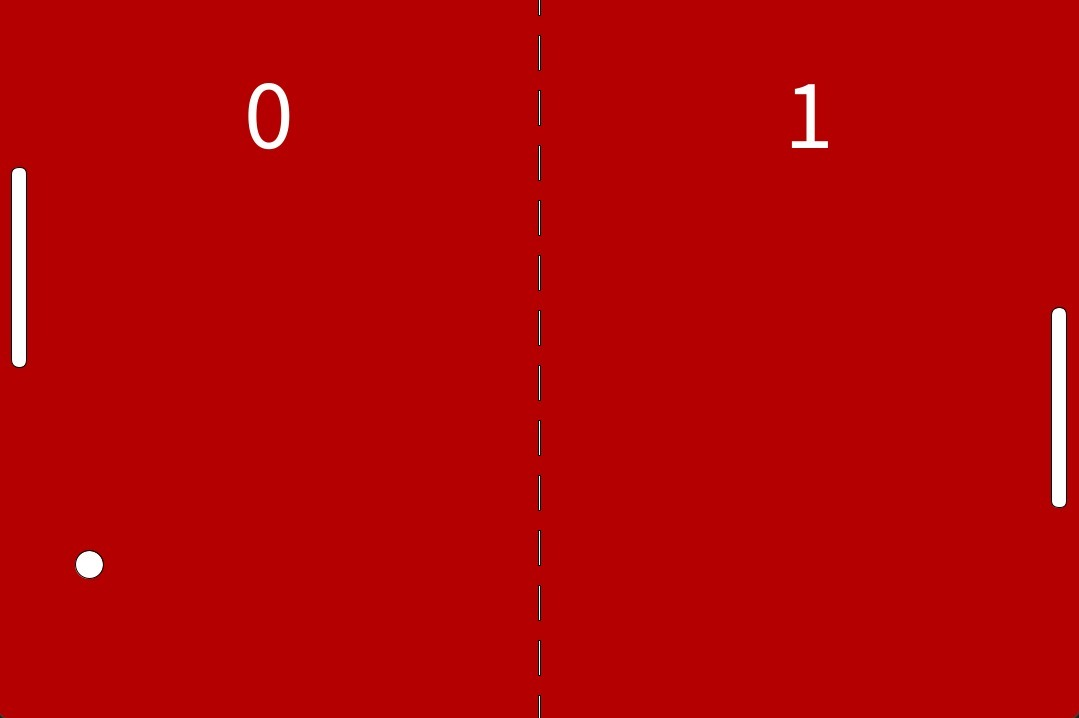
\includegraphics{rodando}}}{VPlayer.swf}


 %*----------- notes__
    \note[item]{Notes can help you to remember important information. Turn on the notes option.}
\end{frame}
%-





